%! Author = Mads Sørensen
%! Date = 14-11-2021

\section{Analyse}
Analysen af opgaven tager udgangspunkt i følgende artefakter; domænemodel, kravspecificering, use case diagram, use case beskrivelser, systemsekvensdiagram, sekvensdiagram.

%! Author = Mads Sørensen
%! Date = 11-11-2021

\section{Kravspecifikation}
Krav er opstillet ud fra den stillet opgave. Vi identificerede først kravene ud fra spilreglerne, som kan kategoriseres som funktionelle krav. Vi havde også ikke-funktionelle krav, som krav til dokumentation, konfiguration osv. Vi havde i projektet stort fokus på at fuldføre de krav, der bragt os tættest på det ønsket produkt.

\begin{table}[H]
   \renewcommand{\arraystretch}{1.5}
   \centering
   \caption{Funktionelle krav} \label{tabel:funkrav}
   \vspace{0.2cm}
   \begin{tabular}{ |p{0.5cm}|p{10cm}|p{2cm}| }
       \hline
       \textbf{ID} & \textbf{Krav} & \textbf{Prioritering} \\
       \hline
       01 & Spillet skal understøtte 2 til 4 spillere & Høj \\
       \hline
       02 & Hver spiller skal starte med $35 & Høj\\
       \hline
       03 & Hver spiller skal starte på startfeltet & Høj\\
       \hline
       04 & Spilleren skal købe et felt, hvis de lander på det, hvis ikke ejet af anden spiller. & Høj \\
       \hline
       05 & Spillere, der lander på et købt felt, skal betale feltets leje til ejeren af feltet. & Høj\\
       \hline
       05A & Spilleren skal betale ejeren dobbelt, hvis ejeren af feltet ejer begge felter af samme farve som det givne felt. & Høj \\
       \hline
       06 & Spillet starter med at hver spiller skal rulle en terning, hvorpå den spiller med det højeste kast starter. & Lav \\
       06A & Hvis flere spillere slår den samme højeste værdi slår de om igen. & \\
       \hline
       07 & Spillet skal bruge GUI’en importeret fra Maven. & Høj \\
       07A & Brættet skal bestå af 24 felter. & \\
       07B & Hver 3. felt der kan købes skal have en farve. & \\
       07C & Hver farve skal have 2 felter som kan købes. & \\
       \hline
       08 & Spillet skal gå på tur, og spilleren slår med 2 terninger & Høj \\
       \hline
       09 & Spillere skal rykke antallet af felter frem lig værdien af terninger. & Høj \\
       \hline
       10 & Spillere skal modtage \$2 ved at passere start & Lav \\
       \hline
       11 & Spillere får en ekstra tur ved at lande på railroad feltet & Lav\\
       \hline
       12 & Spillere betaler \$3 ved at lande på “gå i fængsel” & Lav\\
       \hline
       13 & Spillere skal ændre deres position til “fængsel” når de lander på “Gå i fængsel” & Lav\\
       \hline
       14 & Spillet bør have alle chancekort som vist i det vedhæftede dokument & Lav \\
       \hline
       15 & Spilleren skal betale \$2 til summen af “Loose Change” hvis de lander på “Fireworks” eller “Water show” & Lav \\
       \hline
       16 & Spilleren skal få udbetalt alle opsparede penge når der landes på “loose change” & Lav\\
       \hline
       17 & Hvis man lander man på et chancekortfelt og trækker et kort, der beder spilleren om at bevæge sig til en specifik farve, men farven er komplet optaget af én modstander, skal man trække et nyt kort. & Lav \\
       17A & Hvis der derimod er to spillere, der deles om samme farve, men er placeret i hver deres felt, må man fjerne en spiller og dermed overtage det felt. & \\
       \hline
   \end{tabular}
 \end{table}

\subsection{Use case diagram}
\begin{figure}[H]
    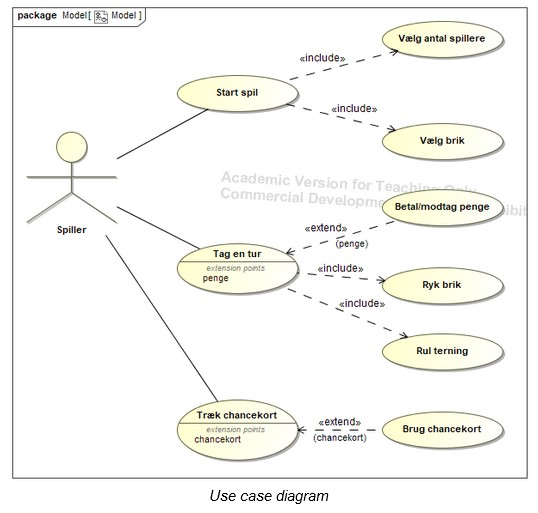
\includegraphics[width=10cm]{figures/usecasediagram}
    \caption{Use case diagram}
\end{figure}

\subsection{Use cases}
Vi har identificeret og analyseret en række use cases i den udleverede opgave. De vigtigste use cases er: \textit{Start spil, Tag tur} og \textit{Træk chancekort}.

\begin{itemize}
    \item \textbf{UC1:} Start spil
    \begin{itemize}
        \item \textbf{UC1.1:} Vælg antal spillere
        \item \textbf{UC1.2:} Tag en tur
    \end{itemize}
    \item \textbf{UC2:} Tag en tur
    \begin{itemize}
        \item \textbf{UC2.1:} Betal/Modtag penge
        \item \textbf{UC2.2:} Ryk brik
        \item \textbf{UC2.3:} Rul terning
    \end{itemize}
    \item \textbf{UC3:} Træk chancekort
    \begin{itemize}
        \item \textbf{UC3.1:} Brug chancekort
    \end{itemize}
\end{itemize}


\textbf{Brief}

\begin{table}[H]
    \renewcommand{\arraystretch}{1.5}
    \centering
    \begin{table}{l{12cm}}
        \hline
        \textbf{ID: UC1} Start spil \\
        \hline
        \textbf{Actor:} Spiller\\
        \hline
        \textbf{Basic flow:} Spiller starter spillet.\\
        \hline
    \end{table}\\
    \begin{table}{l{12cm}}
        \hline
        \textbf{ID: UC1.1} Vælg antal spillere \\
        \hline
        \textbf{Actor:} Spiller\\
        \hline
        \textbf{Basic flow:} Spiller vælger hvor mange spillere der deltager i spillet.\\
        \hline
    \end{tabular}
\end{table}

        ID: UC1.2 Vælg brik \\
        Actor: Spiller \\
        Basic flow: Hver spiller vælger en brik som de får tildelt resten af spillet. \\
        ID: UC2 Tag en tur \\
        Actor: Spiller \\
        Basic flow: Spiller påbegynder tag en tur. \\
        ID: UC2.1 Betal/modtag penge \\
        Actor: Spiller \\
        Basic flow: Spiller betaler en modspiller (eller bank) penge. \\
        ID: UC2.2 Ryk brik \\
        Actor: Spiller \\
        Basic flow: Spiller rykker sin brik antal felter frem på brættet med det antal øjne, terningen viser. \\
        ID: UC2.3 Rul terning \\
        Actor: Spiller \\
        Basic flow: Når det er den pågældende spillers tur, så ruller spilleren terningen, hvorefter en terningsværdi fås. Værdien benyttes til at ændre spillerens position. \\
        ID: UC3 Træk chancekort \\
        Actor: Spiller \\
        Basic flow: Spiller trækker et chancekort, hvorefter et tilfældigt kort modtages. \\
        ID: UC3.1 Brug chancekort \\
        Actor: Spiller \\
        Basic flow: Spiller benytter sit chancekort. \\
        \bottomrule

